\documentclass{beamer}
\usepackage[utf8]{inputenc}
\usetheme{Warsaw}
\usepackage[french]{babel}

\title{Projet de Traitement du Signal\\---\\Segmentation d'image SAR}
\author{Philippe \bsc{Tran Ba} et Élie \bsc{Bouttier}}
\institute{ENSEEIHT, département TR}

\usepackage{xcolor,times}

\usepackage{listings}
  \newcommand*\styleC{\fontsize{9}{10pt}\usefont{T1}{ptm}{m}{n}\selectfont }
  \newcommand*\styleD{\fontsize{9}{10pt}\usefont{OT1}{pag}{m}{n}\selectfont }

  \makeatletter
  % on fixe le langage utilisé
  \lstset{language=matlab}
  \edef\Motscle{emph={\lst@keywords}}
  \expandafter\lstset\expandafter{%
    \Motscle}
  \makeatother


  \definecolor{Ggris}{rgb}{0.45,0.48,0.45}

  \lstset{emphstyle=\rmfamily\color{blue}, % les mots réservés de matlab en bleu
  basicstyle=\styleC,
  keywordstyle=\ttfamily,
  commentstyle=\color{Ggris}\styleD, % commentaire en gris
  numberstyle=\tiny\color{red},
  numbers=left,
  numbersep=10pt,
  lineskip=0.7pt,
  showstringspaces=false}
  %  % inclure le fichier source
  \newcommand{\FSource}[1]{%
  \lstinputlisting[texcl=true]{#1}
  }



\begin{document}

\begin{frame}
\titlepage
\end{frame}

\begin{frame}
\tableofcontents
\end{frame}

\begin{frame}
\section{Introduction}
\begin{itemize}
 \item La segmentation d'images
 \item Image SAR
 \item Bruit speckle
\end{itemize}
\end{frame}

\begin{frame}
\section{Génération d'une ligne d'image SAR}
\subsection{Génération d'une ligne d'image}
\FSource{matlab/genligne.m}
\end{frame}

\begin{frame}
\begin{center}
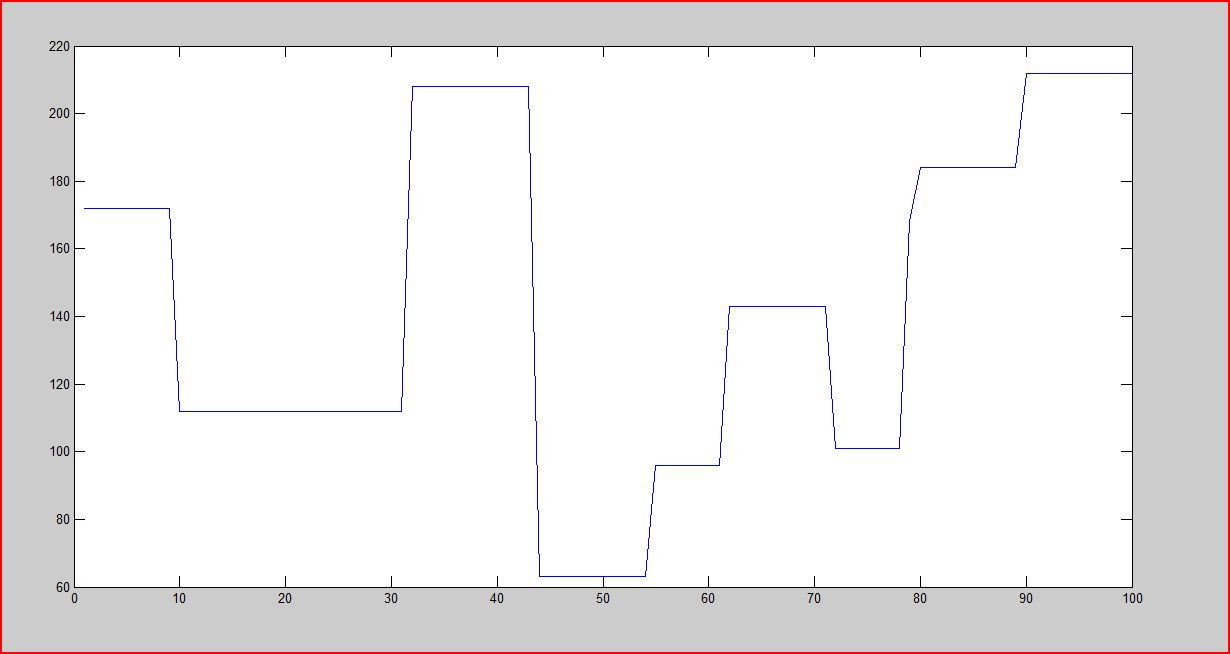
\includegraphics[scale=0.35]{capture/Capturer.JPG}\\
$\mu=1/10, largeur=500, profondeur=256$
\end{center}
\end{frame}

\begin{frame}
\subsection{Génération du bruit}
\FSource{matlab/A.m}
\end{frame}

%\begin{frame}
%\begin{center}
%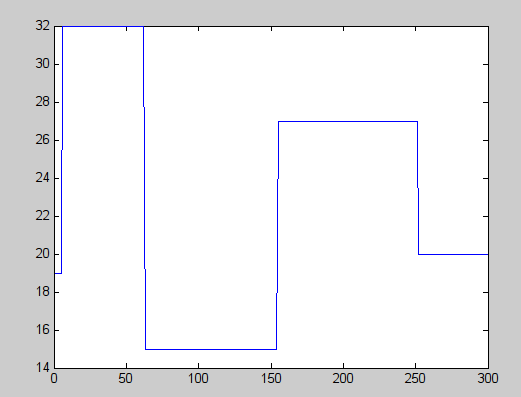
\includegraphics[scale=0.5]{capture/A.png}
%\end{center}
%\end{frame}

\begin{frame}
\subsection{Ligne d'image bruitée}
\begin{center}
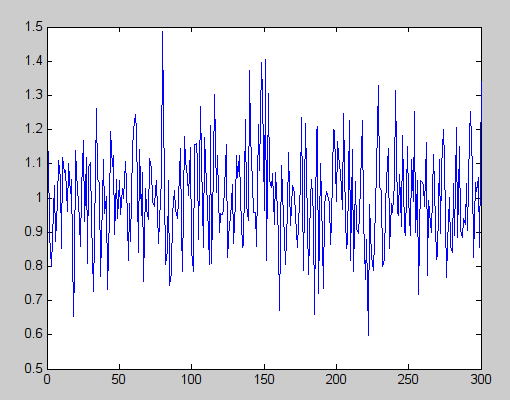
\includegraphics[scale=0.5]{capture/B.png}\\
Bruit speackle
\end{center}
\end{frame}

%\begin{frame}
%\begin{center}
%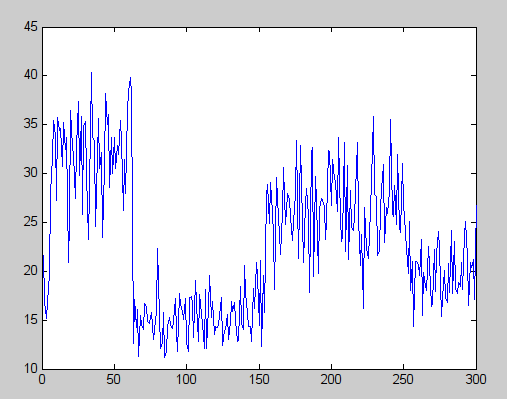
\includegraphics[scale=0.5]{capture/C.png}
%\end{center}
%\end{frame}

\begin{frame}
\begin{center}
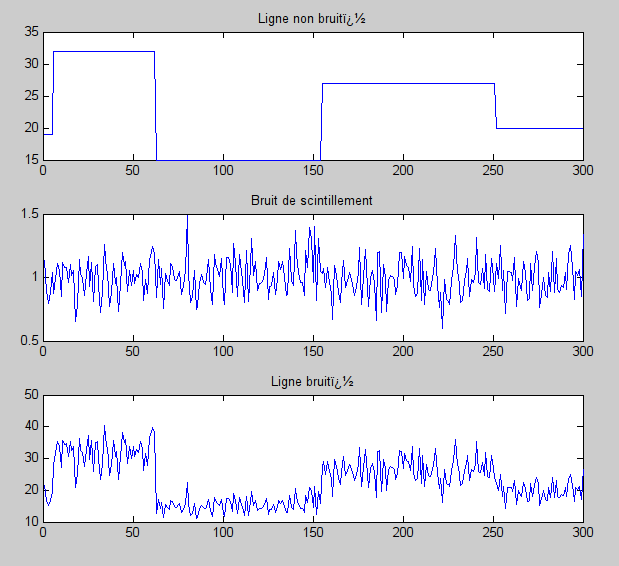
\includegraphics[scale=0.4]{capture/D.png}
\end{center}
\end{frame}

\begin{frame}
\section{Analyse spectrale}
\subsection{Périodogramme et périodogramme cumulé}
\begin{center}
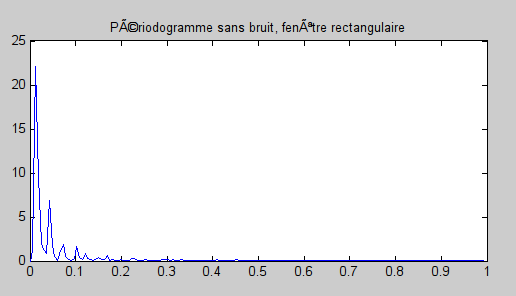
\includegraphics[scale=0.5]{capture/E.png}
\end{center}
\end{frame}

\begin{frame}
\begin{center}
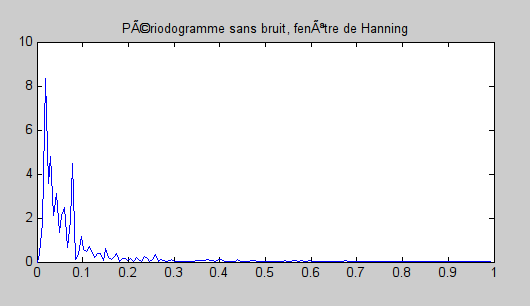
\includegraphics[scale=0.4]{capture/F.png}
\end{center}
\end{frame}

\begin{frame}
\begin{center}
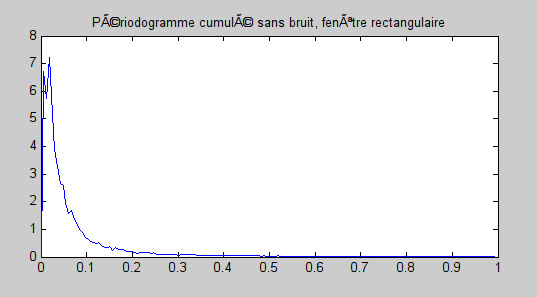
\includegraphics[scale=0.4]{capture/G.png}
\end{center}
\end{frame}

\begin{frame}
\begin{center}
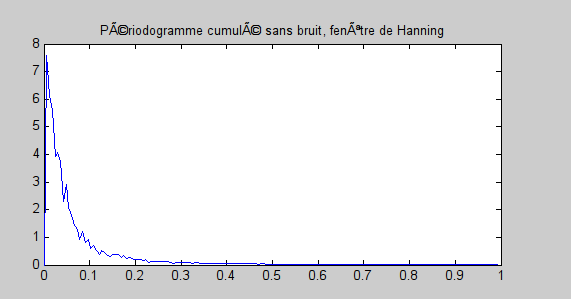
\includegraphics[scale=0.4]{capture/H.png}
\end{center}
\end{frame}

\begin{frame}
\section{Détection de rupture sur une image SAR}
\FSource{matlab/isef.m}
\end{frame}

\begin{frame}
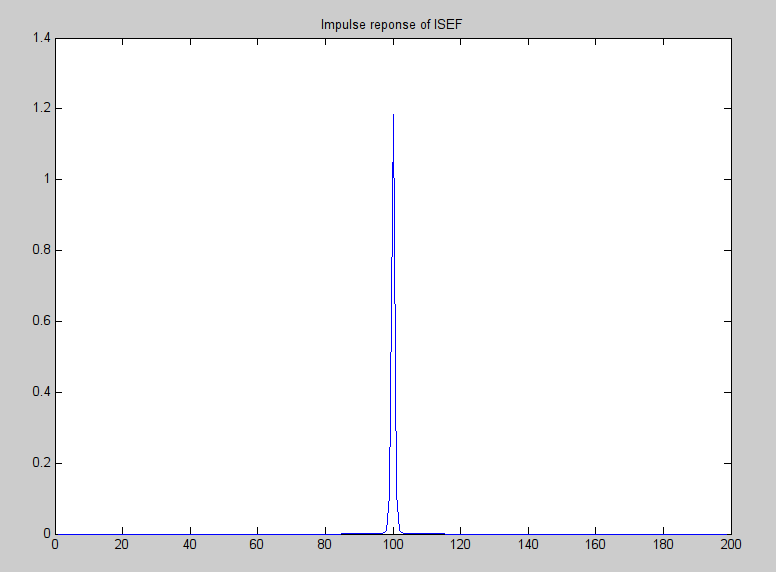
\includegraphics[width=10cm]{capture/filtre.png}
\end{frame}

\begin{frame}
\begin{center}
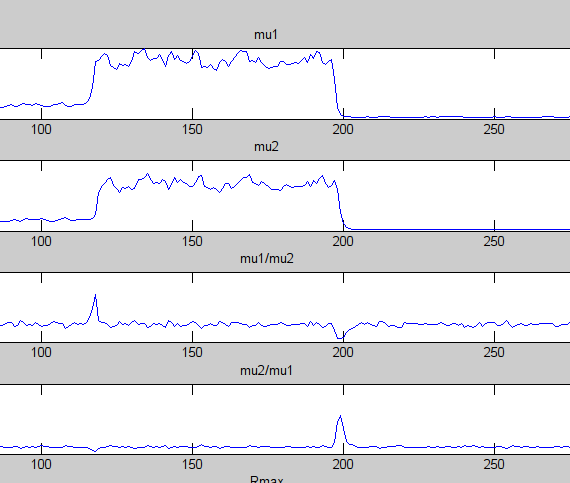
\includegraphics[scale=0.4]{capture/I.png}
\end{center}
\end{frame}

\begin{frame}
\begin{center}
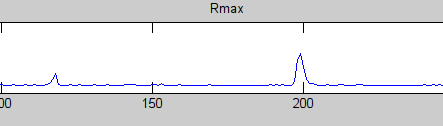
\includegraphics[scale=0.4]{capture/J.png}
\end{center}
\end{frame}

\begin{frame}
\begin{center}
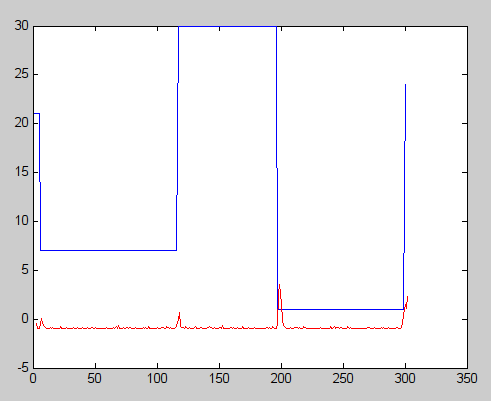
\includegraphics[scale=0.4]{capture/K.png}
\end{center}
\end{frame}

\begin{frame}
\begin{center}
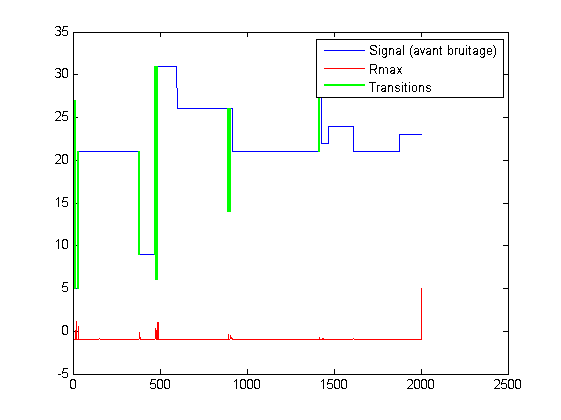
\includegraphics[scale=0.7]{capture3/partie3_07.png}
\end{center}
\end{frame}

\end{document}
